\section{Pulling and inserting a plug}
	\label{sec:plug}
	
	One of the surprise tasks at the DARPA Robotics Challenge consisted of pulling out a plug
	from one socket and putting it back into another socket, in a set-up like the one shown in
	\figurename~\ref{fig:Sockets-Plug}.
	
	\begin{figure}[b]
		\centering
		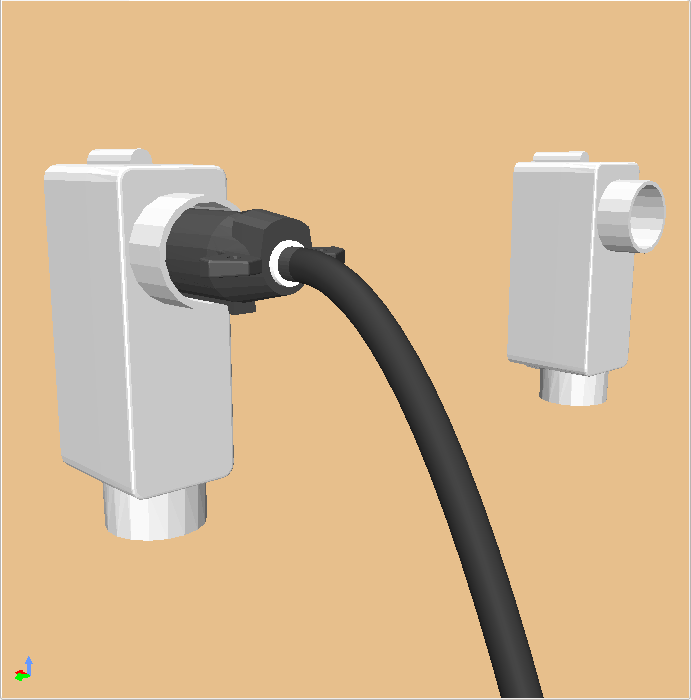
\includegraphics[height = 4cm]{img/Sockets-Plug}
		\caption{Plug Task.}
		\label{fig:Sockets-Plug}
	\end{figure}
	
	\subsection{Detection of the socket and plug}
		
		In order to perform this task it is first necessary to identify the plug and the socket where
		it is originally inserted, by placing the corresponding Manipulation Marker within the poing cloud.
		The reason to identify both objects instead of just the plug is because almost half of it
		is not visible as it is inside of the socket, making it too difficult just to match the plug,
		given the low density of points belonging to it due to its small size.
		
		By using a PCL's built in function it is possible to detect all the planes in the scene,
		one of them being the wall where the sockets are installed.
		Then, given that the front face of the sockets is parallel to this wall, it is possible
		to use the corresponding plane equation to calculate the socket's orientation with respect to
		the robot, in such a way that the plug is directed towards it.
		Having done this, one point belonging to the plug can be manually selected in order to compute
		an approximate initial position for the Manipulation Marker representing the socket and the plug.
		This one is later refined, after the robot has arrived to the desired stance and the point cloud
		has been adjusted by using the robot's hands as a reference, as seen in
		\figurename~\ref{fig:SocketPlugMarker} (and explained in Subsection~\ref{sub:uncertainties}).
		
		\begin{figure}[t]
			\centering
			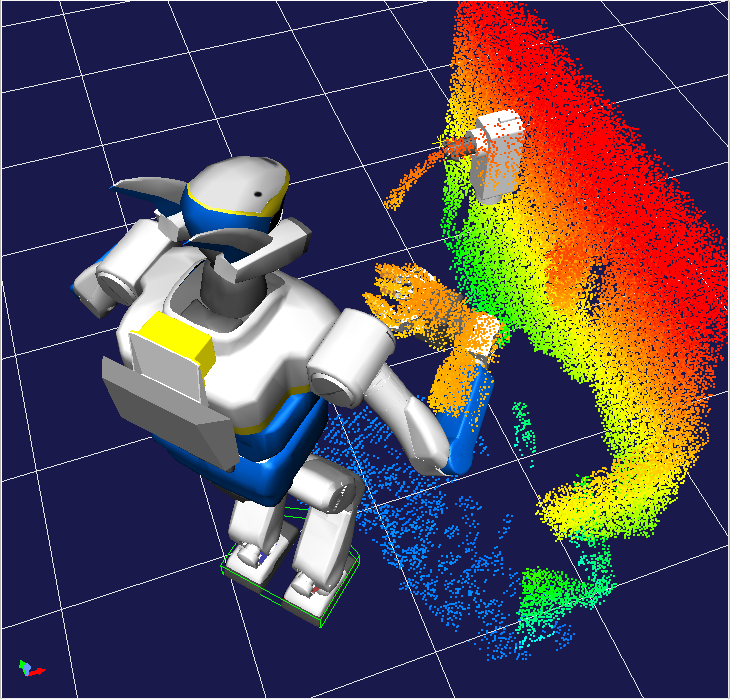
\includegraphics[height = 5cm]{img/SocketPlugMarker}
			\caption{Detection of the socket and the plug.}
			\label{fig:SocketPlugMarker}
		\end{figure}
		
	\subsection{Grasping the plug}
		
		Having detected an approximate attitude for the socket, the robot first approaches the plug
		with one hand while aligning the camera installed at the other hand with the axis of the plug.
		This is to be able to make slight adjustments of the grasping hand by using visual feedback.
		
		The size of the visible part of the plug is not that big compared to the hand of the robot,
		and because of that the tolerance for	grasping the plug is minimum.
		Then, it is required to grasp the plug at the point in which the medial side of the hand
		touches the cylindrical shaped part of the socket.
		This can be done by reducing the angle of the gripper and then, by moving the hand along the
		axis of the plug until sensing 30 N of force (enough for considering that it arrived to the socket).
		This configuration of the robot just before moving the hand towards to the socket is depicted in
		\figurename~\ref{fig:PreCloseHand}.
		
		\begin{figure}[t]
			\centering
			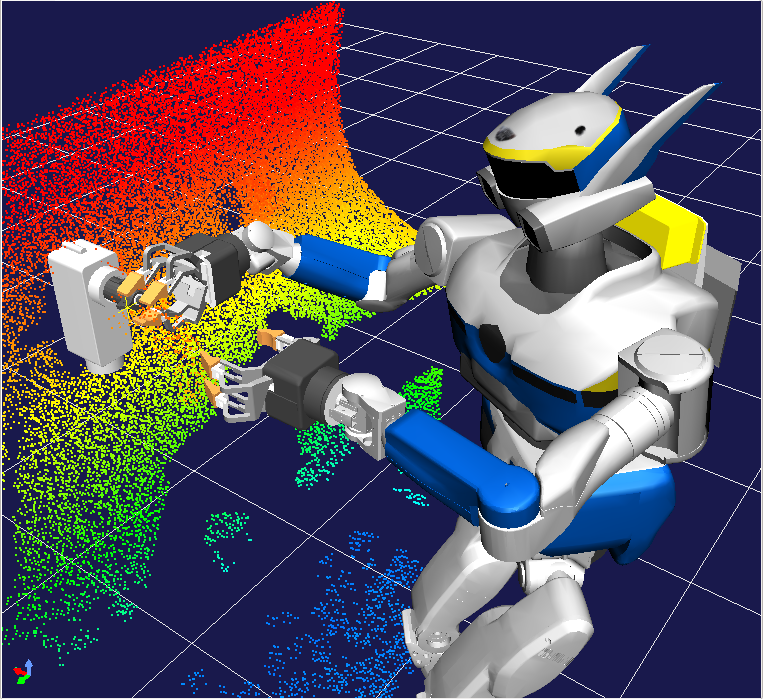
\includegraphics[height = 5cm]{img/PreCloseHand}
			\caption{Configuration of the robot before grasping the plug.}
			\label{fig:PreCloseHand}
		\end{figure}
		
		This strategy is very effective (when adjusted properly) as the grasp can be done every time at the
		desired point even in the presence of uncertainties, as shown in the dynamical simulation depicted
		in \figurename~\ref{fig:GraspPlug}.
		
		\begin{figure}[b]
			\centering
			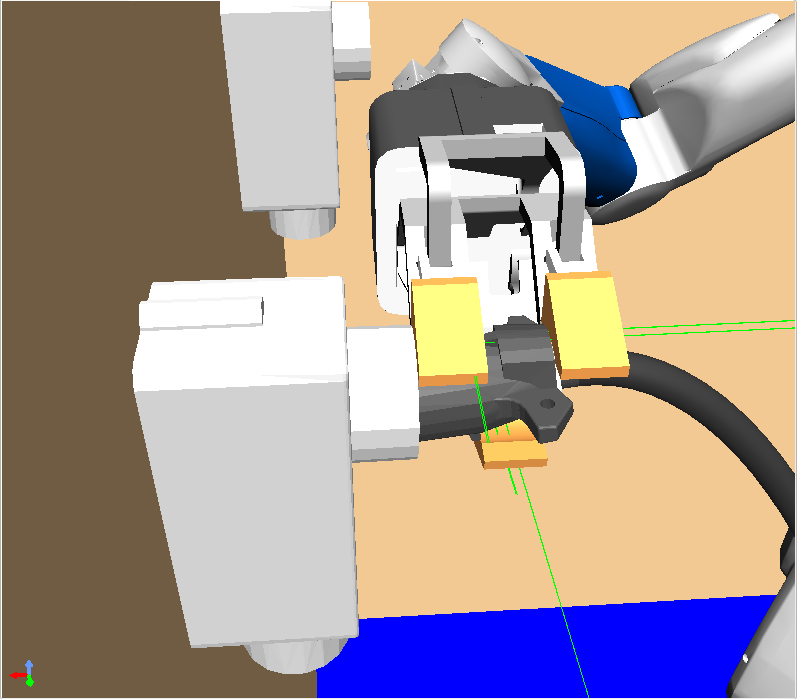
\includegraphics[height = 5cm]{img/GraspPlug}
			\caption{The plug being effectively grasped at the desired point.}
			\label{fig:GraspPlug}
		\end{figure}
		
	\subsection{Pulling and adjusting the plug}
		
		After grasping the plug, the robot pulls the plug.
		Due to the balancing process this motion may not be performed exactly along the axis of the plug,
		and it may hit the inner walls of the socket, modifying the planned relative attitude between the
		plug and the hand.
		
		For this reason, before inserting the plug into the other socket, the robot first brings the plug
		in front of its chest, takes an updated point cloud, and uses the camera placed at the head and
		at the other hand to look at the plug from two perpendicular directions, as seen in
		\figurename~\ref{fig:WatchPlug}.
		By using this information it is possible to fix the actual attitude of the plug with respect to
		the hand.
		
		\begin{figure}[t]
			\centering
			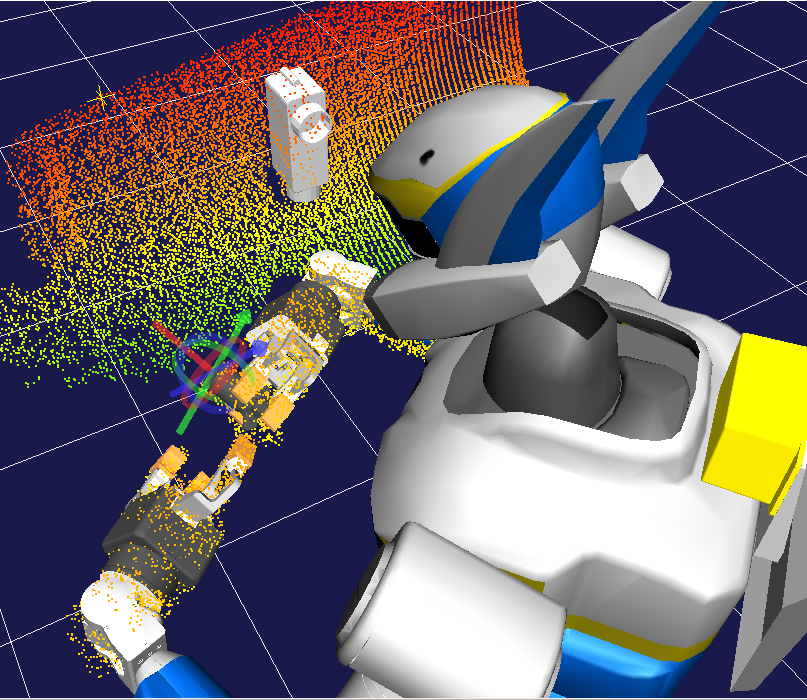
\includegraphics[height = 5cm]{img/WatchPlug}
			\caption{After pulling the plug its attitude is adjusted.}
			\label{fig:WatchPlug}
		\end{figure}
		
	\subsection{Inserting the plug}
		
		Once the Manipulation Marker representing the plug is fixed at the hand, it can further be properly
		aligned with the destination socket.
		This one can be represented with another marker (Object Marker), which can be adjusted within the
		point cloud before taking the plug to the pre-insertion position.
		However, because of inaccuracies of the point cloud, the camera at the other hand is used once again
		together with the camera at the head to look at the plug, and use this visual feedback to adjust its
		position to properly insert the plug within few movements.
		This is represented in \figurename~\ref{fig:InsertPlug}.
		
		\begin{figure}[b]
			\centering
			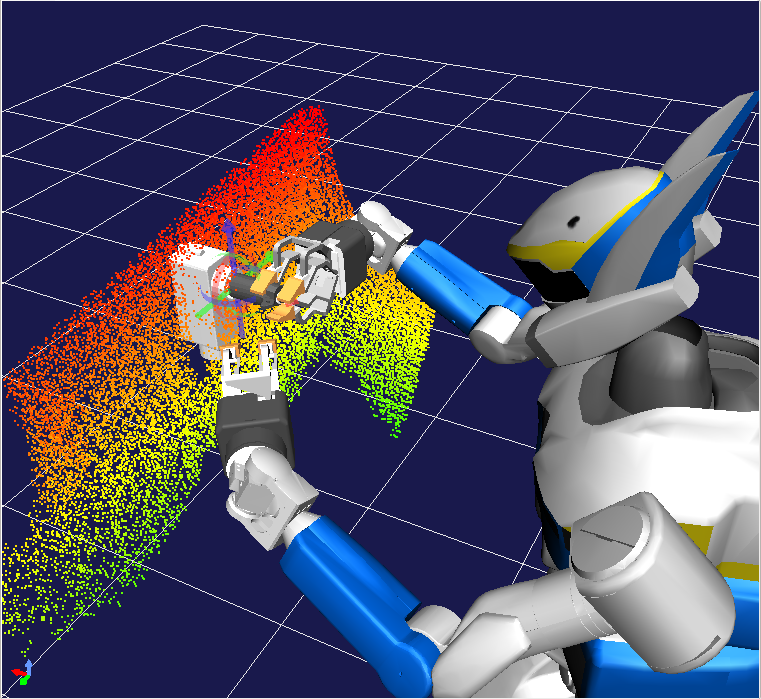
\includegraphics[height = 5cm]{img/InsertPlug}
			\caption{The plug is inserted by using visual feedback.}
			\label{fig:InsertPlug}
		\end{figure}
		
		Then, once the task is completed, the hand opens and an updated point cloud is taken, in order to
		correctly plan the returning motion without hitting the cable of the plug.